%%%%%%%%%%%%%%%%%%%%%%%%%%%%%%%%%%%%%%%%%%%%%%%%%%%%%%%%%%%%%%%%%%%%%%%%%%%
%
% Template for a LaTex article in Slovak.
%
%%%%%%%%%%%%%%%%%%%%%%%%%%%%%%%%%%%%%%%%%%%%%%%%%%%%%%%%%%%%%%%%%%%%%%%%%%%

\documentclass{article}

\usepackage[utf8]{inputenc}
\usepackage[slovak]{babel}
\usepackage[document]{ragged2e}
\usepackage{amsmath}
\usepackage{siunitx}
\usepackage{multicol}
\usepackage{textcomp}
\usepackage{amsmath, amsthm, amsfonts}
\usepackage{graphicx}
\usepackage{url}
\usepackage{subcaption}
\usepackage{float}
% Theorems
%-----------------------------------------------------------------
\newtheorem{thm}{Theorem}[section]
\newtheorem{cor}[thm]{Corollary}
\newtheorem{lem}[thm]{Lemma}
\newtheorem{prop}[thm]{Proposition}
\theoremstyle{definition}
\newtheorem{defn}[thm]{Definition}
\theoremstyle{remark}
\newtheorem{rem}[thm]{Remark}

% Shortcuts.
% One can define new commands to shorten frequently used
% constructions. As an example, this defines the R and Z used
% for the real and integer numbers.
%-----------------------------------------------------------------
\def\RR{\mathbb{R}}
\def\ZZ{\mathbb{Z}}

% Similarly, one can define commands that take arguments. In this
% example we define a command for the absolute value.
% -----------------------------------------------------------------
\newcommand{\abs}[1]{\left\vert#1\right\vert}

% Operators
% New operators must defined as such to have them typeset
% correctly. As an example we define the Jacobian:
% -----------------------------------------------------------------
\DeclareMathOperator{\Jac}{Jac}

%-----------------------------------------------------------------
\title{Zadanie 2}
\author{Miroslav Kurka\\
  \small Dept. of Biophysics\\
  \small Pavol Jozef Šafárik University in Košice\\
  \small Slovakia 
}

\begin{document}
\maketitle


\section{Úloha}
Numericky riešte problém ideálneho kyvadla hmotnosti m, pripevneného k pevnému čapu tuhou tyčou dĺžky L (viď obrázok a prednášky). Predpokladajme, že uhol vychýlenia $\theta$ je malý, takže platí $\sin(\theta) \cong \theta$. V takom prípade je možné popísať pohyb kyvadla sústavou diferenciálnych rovníc


$$\frac{d\omega}{dt}=-\frac{g}{L}\theta$$
$$\frac{d\theta}{dt}=\omega$$

Vyriešte úlohu pre $t\in[0,20]$ s počiatočnými podmienkami $\theta(0)=0.1$ a $\omega(0)=0$ a krokom $\Delta t= 0.02$ pomocou metód nižšie. Porovnajte výsledky s výsledkami získanými pomocou funkcie lsode(). Výsledky zobrazte v grafe. 
\begin{itemize}
    \item Eulorovou metódou
    \item Metódou Runge-Kutta 4. rádu
    \item lsode()
\end{itemize}

\subsection{Teória}\label{sec:nothing}
Úloha je založená na riešení diferenciálnej rovnice pomocou Runge-Kutta (RK) metód. Tie používajú aproximaciu derivacií kombináciou hodnôt funkcie $f$ v niekoľkých strategických bodoch na intervale $[t_n, t_{n+1}]$\cite{Zukovic}. Všeobecne sú dané rekurentným vzťahom:
\begin{equation}
    y_{n+1}=y_n+h_n\sum_{i=1}^r \alpha_i k_i
\end{equation}
\subsubsection{Eulerova metóda}
Jedná sa o RK metódu prvého rádu. Metóda je založená na princípe nahradenia krivky $y=f(x)$ jej dotyčnicou v bode $[x_i,f(x_i)]$ na intervale $⟨x_i,x_i+1⟩$. Keďže smernicu dotyčnice vieme vypočítať pomocou derivácie funkcie t.j. $k=y'(x_i)=f(x_i,y_i)$, dostávame rekurentný vzorec pre výpočet hodnoty funkcie v bode $y_{i+1}$\cite{Web}:

\begin{equation}
y_{i+1}=y_i+h f(x_i,y_i)
\end{equation}


kde $h = x_{i+1}-x_i$ je krok metódy.

Podľa rovnice 2.23 z knihy \cite{Zukovic} je možné metódu zapísať v maticovej forme pre našu sústavu dvoch rovníc popisujúcich pohyb kyvadla:


\begin{equation}
    \mathbf{x}_{i+1} = \mathbf{x}_{i} + \Delta t \cdot \mathbf{V} \cdot \mathbf{x}_{i}
\end{equation}
kde $\mathbf{V}$ je rovné:

\begin{equation}
    \mathbf{V} = \begin{pmatrix}
    0 & 1 \\
    -\frac{g}{L} & 0
    \end{pmatrix}
\end{equation}
\subsubsection{RK metóda 4. rádu}
Runge-Kuttova metóda 4. stupňa (RK4) je vylepšenie jednoduchšej Eulerovej metódy, ktorá používa iba jedno odhadnutie sklonu funkcie na začiatku každého kroku na aktualizáciu riešenia.


RK4 je metóda vyššieho stupňa, čo znamená, že používa štyri odhady (nazvané $k_1$, $k_2$, $k_3$ a $k_4$) v rôznych bodoch v každom kroku na zlepšenie presnosti riešenia. Tie sa používajú na aktualizáciu riešenia v každom kroku.\cite{Zukovic}
\begin{equation}
    x_{n+1}= x_n + h_n \frac{k_1+2k_2+2k_3+k_4 }{6}
\end{equation}
, kde
$$k_1=f(t_n,x_n)$$
$$k_2=f(t_n+\frac{h_n}{2},x_n+\frac{h_n}{2}k_1)$$
$$k_3=f(t_n+\frac{h_n}{2},x_n+\frac{h_n}{2}k_2)$$
$$k_4=f(t_{n+1},x_n+{h_n}k_3)$$

\subsection{Výsledky}
Na Obr.\ref{fig:dx001} sú zobrazene riešenia pre úlohy. Výsledkom sú zmeny uhla $\theta$ v čase t, kde $\theta$ predstavuje vychýlenie kyvadla. Os x zobrazuje čas t v sekundách. Os y popisuje veľkosť uhla vychýlenia v radiánoch. Najväčšie nadobúdane hodnoty sú 1 a -1 rad, ktoré sa opakujú s periódou. 
\begin{figure}[H]
  \centering
  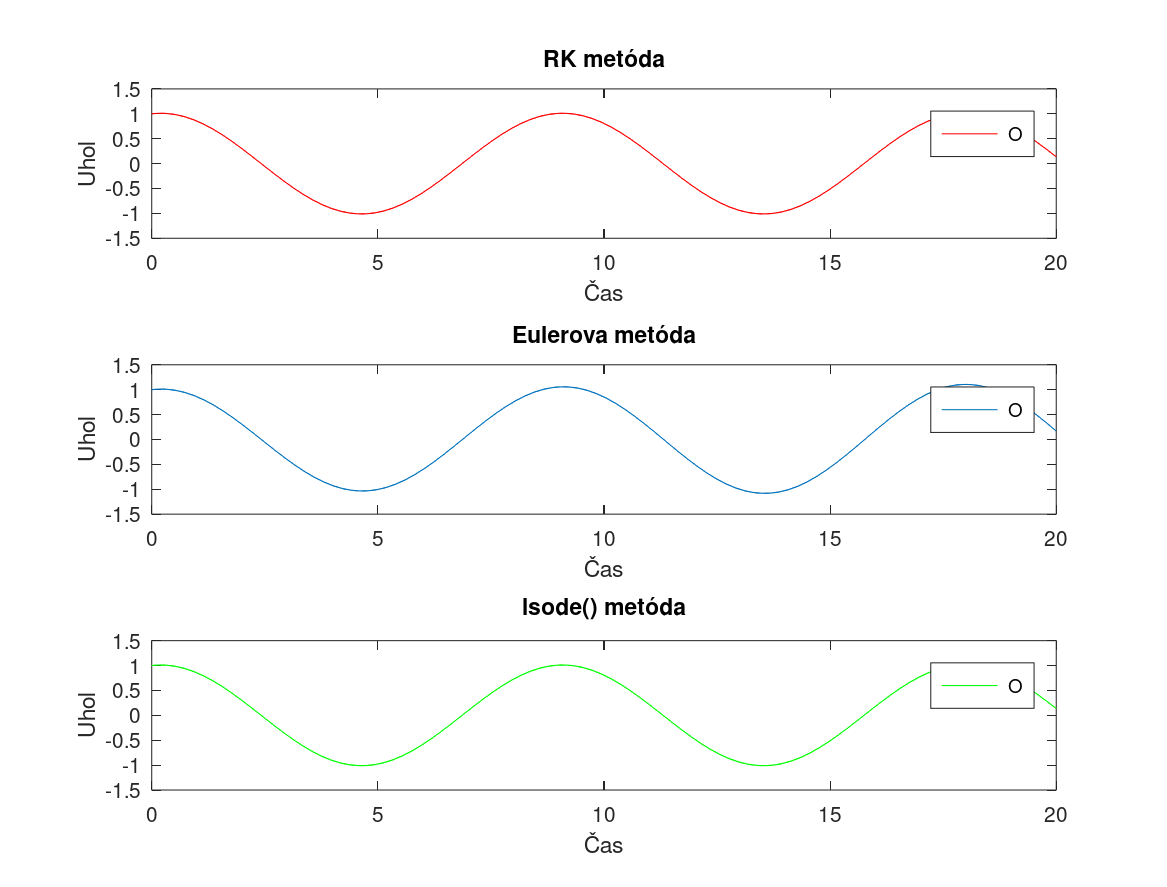
\includegraphics[width=1\textwidth]{graph_hw2.png}
  \caption{Graf ukazuje porovnanie presnosti metód, v prvom prípade sú zobrazené hodnoty pre uhla $\theta$ a v druhom prípade pre uhlovú rýchlosť $\omega$. Modrá prerušovaná čiara označuje Eulorovú metódu, ktorá je najmenej presná. Zelená bodkovaná čiara lsode() vstavanú funkciu a červená plná čiara Runge-Kuttovu metódu 4. rádu.
  }
  \label{fig:dx001}
\end{figure}





\subsection{Záver a diskusia}

Z teórie vyplýva, že presnosť riešenia by sa mala líšiť podlá toho akú metódu zvolíme. Najmenej presná je Eulerova metóda. Následne o niečo presnejšia Runge-Kutte metóda 4. radu a najpresnejšia vstavaná lsode() funkcia.

\pagebreak
% Bibliography
%-----------------------------------------------------------------
\begin{thebibliography}{99}
\bibitem{Web} \emph{Eulerova a Heunova metóda} Dostupné z \url{http://matematikabezproblemov.webjet.sk/domov/studijne-materialy/matematika-vs/numericka-matematika/eulerova-heunova-metoda/}
\bibitem{Zukovic}Žukovič, M. (2015) \emph{Počítačová fyzika I} Dostupné z \url{https://ufv.science.upjs.sk/zukovic/download/POF1/Literatura/Pocitacova%20fyzika%20I.pdf}
\end{thebibliography}

\end{document}
